% ============================================================
%  CS301 - Computer Networks | Team 9 Final Presentation (Beamer)
%  Observability-Aware Trust-Based Grayhole Detection for UASNs
%  Images are read from the figs/ folder.
% ============================================================
\documentclass[aspectratio=169,11pt]{beamer}

\usetheme{Madrid}
\setbeamertemplate{navigation symbols}{}

% Footer: team | title | slide number (no date)
\setbeamertemplate{footline}{%
  \leavevmode%
  \hbox{%
    \begin{beamercolorbox}[wd=.3\paperwidth,ht=2.25ex,dp=1ex,center]{author in head/foot}%
      \usebeamerfont{author in head/foot}\insertshortauthor
    \end{beamercolorbox}%
    \begin{beamercolorbox}[wd=.6\paperwidth,ht=2.25ex,dp=1ex,center]{title in head/foot}%
      \usebeamerfont{title in head/foot}\insertshorttitle
    \end{beamercolorbox}%
    \begin{beamercolorbox}[wd=.1\paperwidth,ht=2.25ex,dp=1ex,right]{date in head/foot}%
      \usebeamerfont{date in head/foot}\insertframenumber{} / \inserttotalframenumber\hspace*{2ex}
    \end{beamercolorbox}}%
  \vskip0pt%
}

\usepackage{booktabs}
\usepackage{xcolor}
\usepackage{amsmath}
\graphicspath{{figs/}}

\definecolor{bad}{RGB}{192,57,43}
\definecolor{good}{RGB}{30,132,73}

\title[Grayhole Detection in UASNs]{Observability-Aware Trust-Based Grayhole Detection\\for Underwater Acoustic Networks}
\subtitle{CS301 Computer Networks Mini Project, Team 9}
\author[Team 9]{\texorpdfstring{\small
  \begin{tabular}{lll}
    241CS110 & Appaji Nagaraja Dheeraj & appajidheeraj.241cs110@nitk.edu.in\\
    241CS111 & Aryan Bokolia & aryanbokolia.241cs111@nitk.edu.in\\
    241CS117 & Karthikeya Gupta & karthikeyagupta.241cs117@nitk.edu.in
  \end{tabular}}{Team 9}}
\institute[NITK]{Department of Computer Science and Engineering\\
National Institute of Technology Karnataka, Surathkal}
\date{}

\begin{document}

% ---------------- 1. Title ----------------
\begin{frame}
  \titlepage
\end{frame}

% ---------------- 2. Problem ----------------
\begin{frame}{Problem statement}
  \begin{itemize}\setlength\itemsep{0.5em}
    \item In an underwater acoustic network, sensors send data to the sink through relays (network layer).
    \item A \textbf{grayhole} relay drops a part of the packets that it must forward (here 30\%). Its loss looks like normal link loss.
    \item The \textbf{watchdog} listens for each forward and accuses a relay with too many misses.
  \end{itemize}

  \vspace{0.6em}
  \begin{block}{A forward is missing when}
    \begin{columns}[t]
      \column{0.24\textwidth}\centering{\color{bad}\Large\bfseries 1}\\\small the relay \textbf{dropped} it\\{\scriptsize (the attack)}
      \column{0.24\textwidth}\centering{\Large\bfseries 2}\\\small the monitor was \textbf{transmitting}\\{\scriptsize (half-duplex)}
      \column{0.24\textwidth}\centering{\Large\bfseries 3}\\\small the packet \textbf{collided} at the relay
      \column{0.24\textwidth}\centering{\Large\bfseries 4}\\\small the \textbf{long link} lost it
    \end{columns}
    \vspace{0.3em}
  \end{block}

  \vspace{0.4em}
  \centering
  Only cause 1 is an attack. Causes 2 to 4 increase with traffic,\\
  so a fixed threshold \textcolor{bad}{\textbf{accuses honest relays}}.
\end{frame}

% ---------------- 3. Proposed approach ----------------
\begin{frame}{Proposed approach}
  \begin{columns}[t]
    \column{0.32\textwidth}
      \begin{block}{1. Observability filter}
        \small A monitor counts a watch window only if it could hear the forward:
        it did not transmit, the relay did not transmit, and no known frame arrived at the relay.
      \end{block}
    \column{0.32\textwidth}
      \begin{block}{2. Expected forwards}
        \small Each link has an expected loss from its distance and the median loss of other links of similar length.\\[0.3em]
        $\text{Trust}_B = \dfrac{\sum \text{heard}}{\sum \text{expected}}$
      \end{block}
    \column{0.32\textwidth}
      \begin{block}{3. Decision at the sink}
        \small Dynamic threshold, baseline cleaning, and a suspect only after two flagged 30-min rounds in a row.
      \end{block}
  \end{columns}

  \vspace{1em}
  \begin{alertblock}{Improvement over the baselines}
    The fixed watchdog counts every silence as a drop. The CAD-style detector uses an average collision rate.
    Our detector excludes each window that the monitor could not observe, and needs no probe packets.
  \end{alertblock}
\end{frame}

% ---------------- 4. Architecture ----------------
\begin{frame}{Architecture}
  \centering
  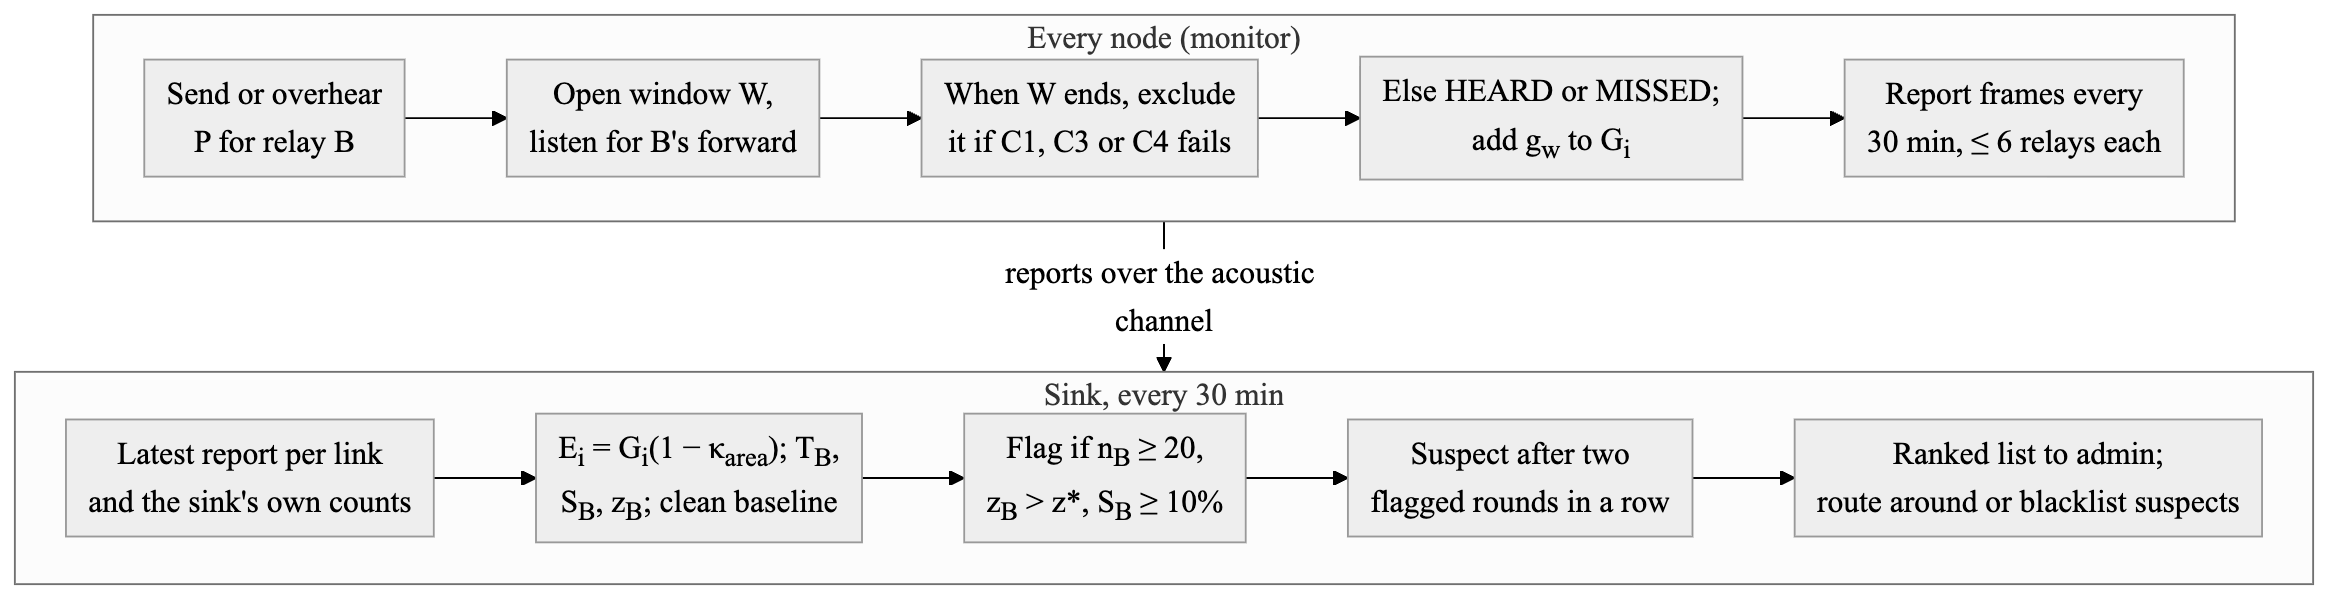
\includegraphics[width=\textwidth]{fig_arch_final.png}

  \vspace{0.8em}
  \small
  \begin{tabular}{@{}ll@{}}
    \toprule
    Simulator & UnetStack 7.0.0 (Groovy agents), 20 sensors and one sink, 4 km $\times$ 4 km\\
    Classes & \texttt{MonitorNode}, \texttt{Detectors}, \texttt{Topology}, \texttt{DistanceLossChannel}\\
    Fair test & Thresholds tuned on topologies 101 to 106, tested on topologies 201 to 210\\
    \bottomrule
  \end{tabular}
\end{frame}

% ---------------- 5. Results: blacklisting ----------------
\begin{frame}{Results: delivery ratio with blacklisting}
  \centering
  {\small \textbf{Delivery ratio} = data packets from honest sensors that reach the sink $\div$ data packets they generate.}\\[0.2em]
  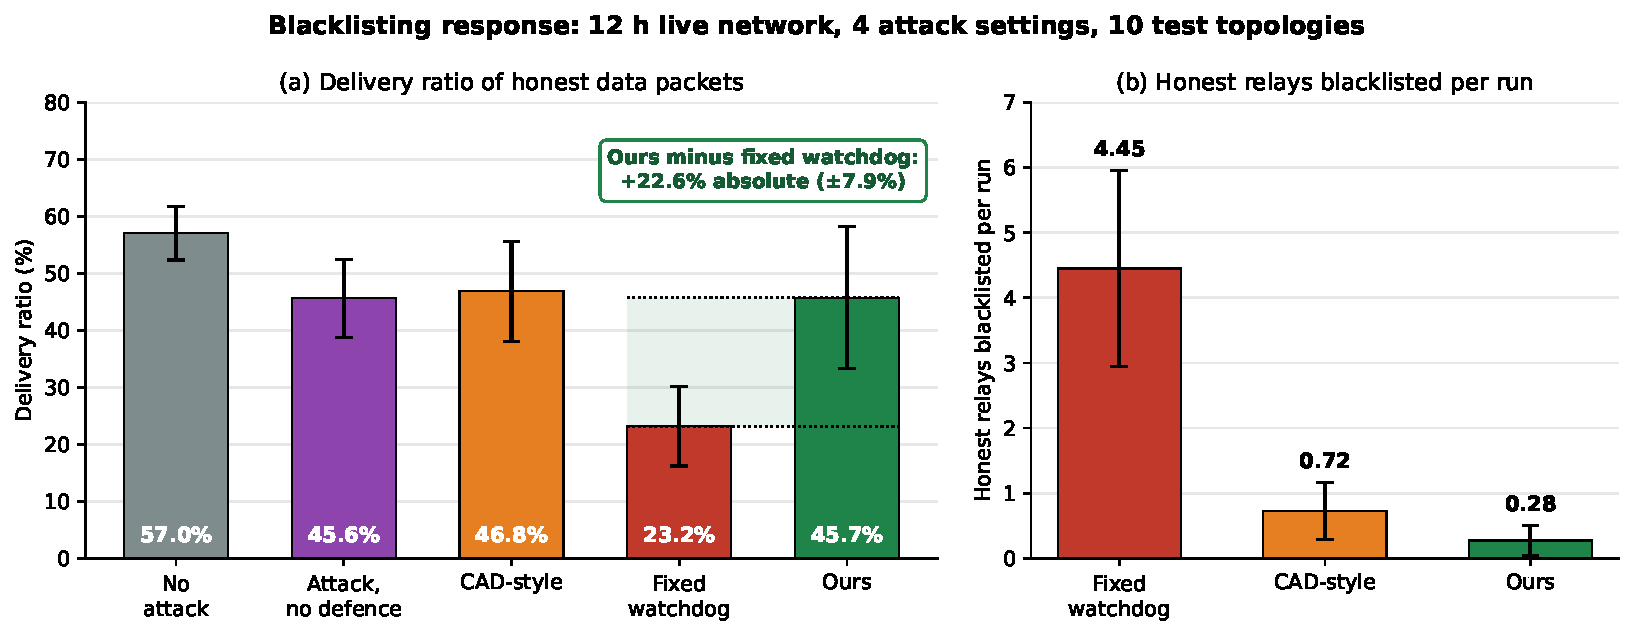
\includegraphics[width=0.88\textwidth]{blacklist.pdf}

  \vspace{0.1em}
  \small
  With the fixed watchdog, the delivery ratio is \textcolor{bad}{\textbf{23.2\%}}. With ours, it is \textcolor{good}{\textbf{45.7\%}}.\\
  Absolute increase: \textbf{22.6\%} ($\pm$7.9\%), because ours blacklists 0.28 honest relays per run and the fixed watchdog 4.45.
\end{frame}

% ---------------- 6. Results: detection ----------------
\begin{frame}{Results: false accusations}
  \begin{columns}[c]
    \column{0.54\textwidth}
      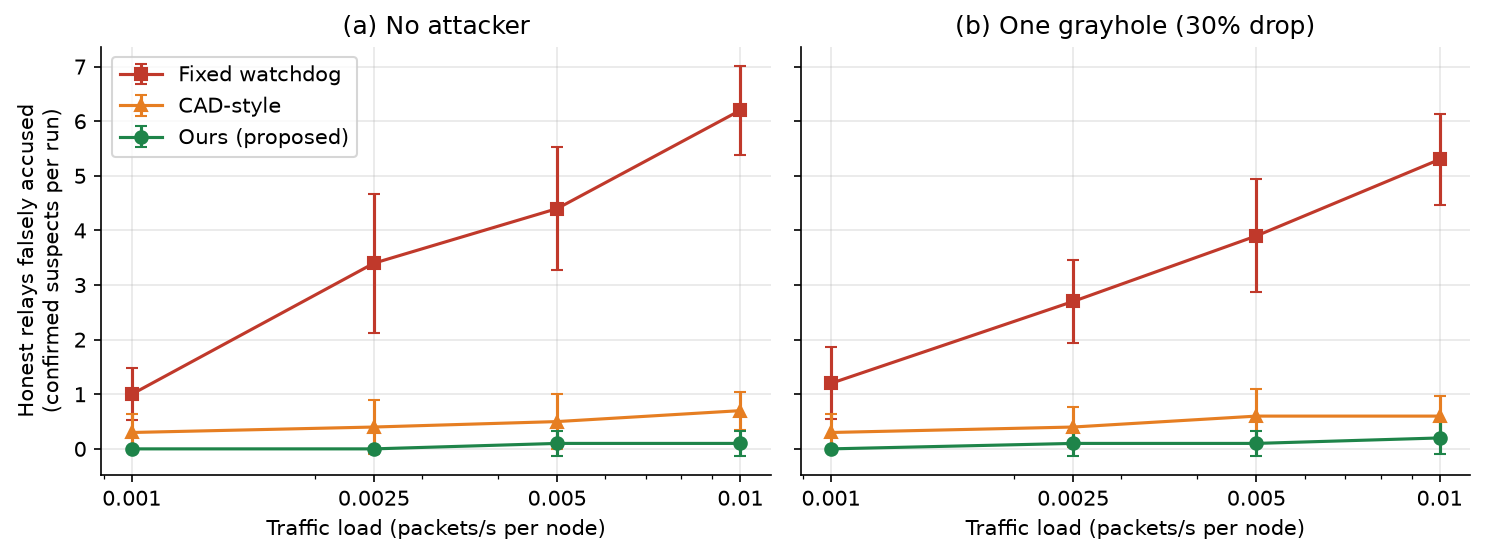
\includegraphics[width=\textwidth]{fig2_false_accusations.png}\\
      {\scriptsize Honest relays accused per run as the traffic load changes}
    \column{0.42\textwidth}
      \footnotesize
      \textbf{Live network, 12 h}\\[0.3em]
      \begin{tabular}{@{}lrr@{}}
        \toprule
        Method & Caught & \shortstack[r]{Honest relays\\accused per run}\\
        \midrule
        Fixed watchdog & 100\% & \textcolor{bad}{7.2}\\
        CAD-style & 58\% & 0.8\\
        \textbf{Ours} & \textbf{95\%} & \textcolor{good}{\textbf{0.3}}\\
        \bottomrule
      \end{tabular}
  \end{columns}
\end{frame}

% ---------------- 7. Conclusion ----------------
\begin{frame}{Conclusion}
  \begin{itemize}\setlength\itemsep{0.5em}
    \item Under water, a missing forward is often not an attack.
    \item Our detector judges only the windows that the monitor could observe, and compares them with the expected loss of each link.
    \item It caught 95\% of the grayholes and accused 0.3 honest relays per run. The fixed watchdog accused 7.2.
    \item With blacklisting, it kept a delivery ratio of 45.7\%. The fixed watchdog kept 23.2\%.
    \item Future work: dishonest monitors, mobile nodes, and learning the loss curve during operation.
  \end{itemize}

  \vspace{1em}
  \centering
  {\Large\bfseries Thank you}
\end{frame}

\end{document}
